%\vspace{-1em}
\section{Experiments}
%\vspace{-0.5em}
\subsection{Simulation Experiment}
%\vspace{-0.5em}
%\begin{figure}[t]
%    \centering
%    \begin{minipage}[t]{0.75\textwidth}
%        \centering
%        \vspace{0pt}
%        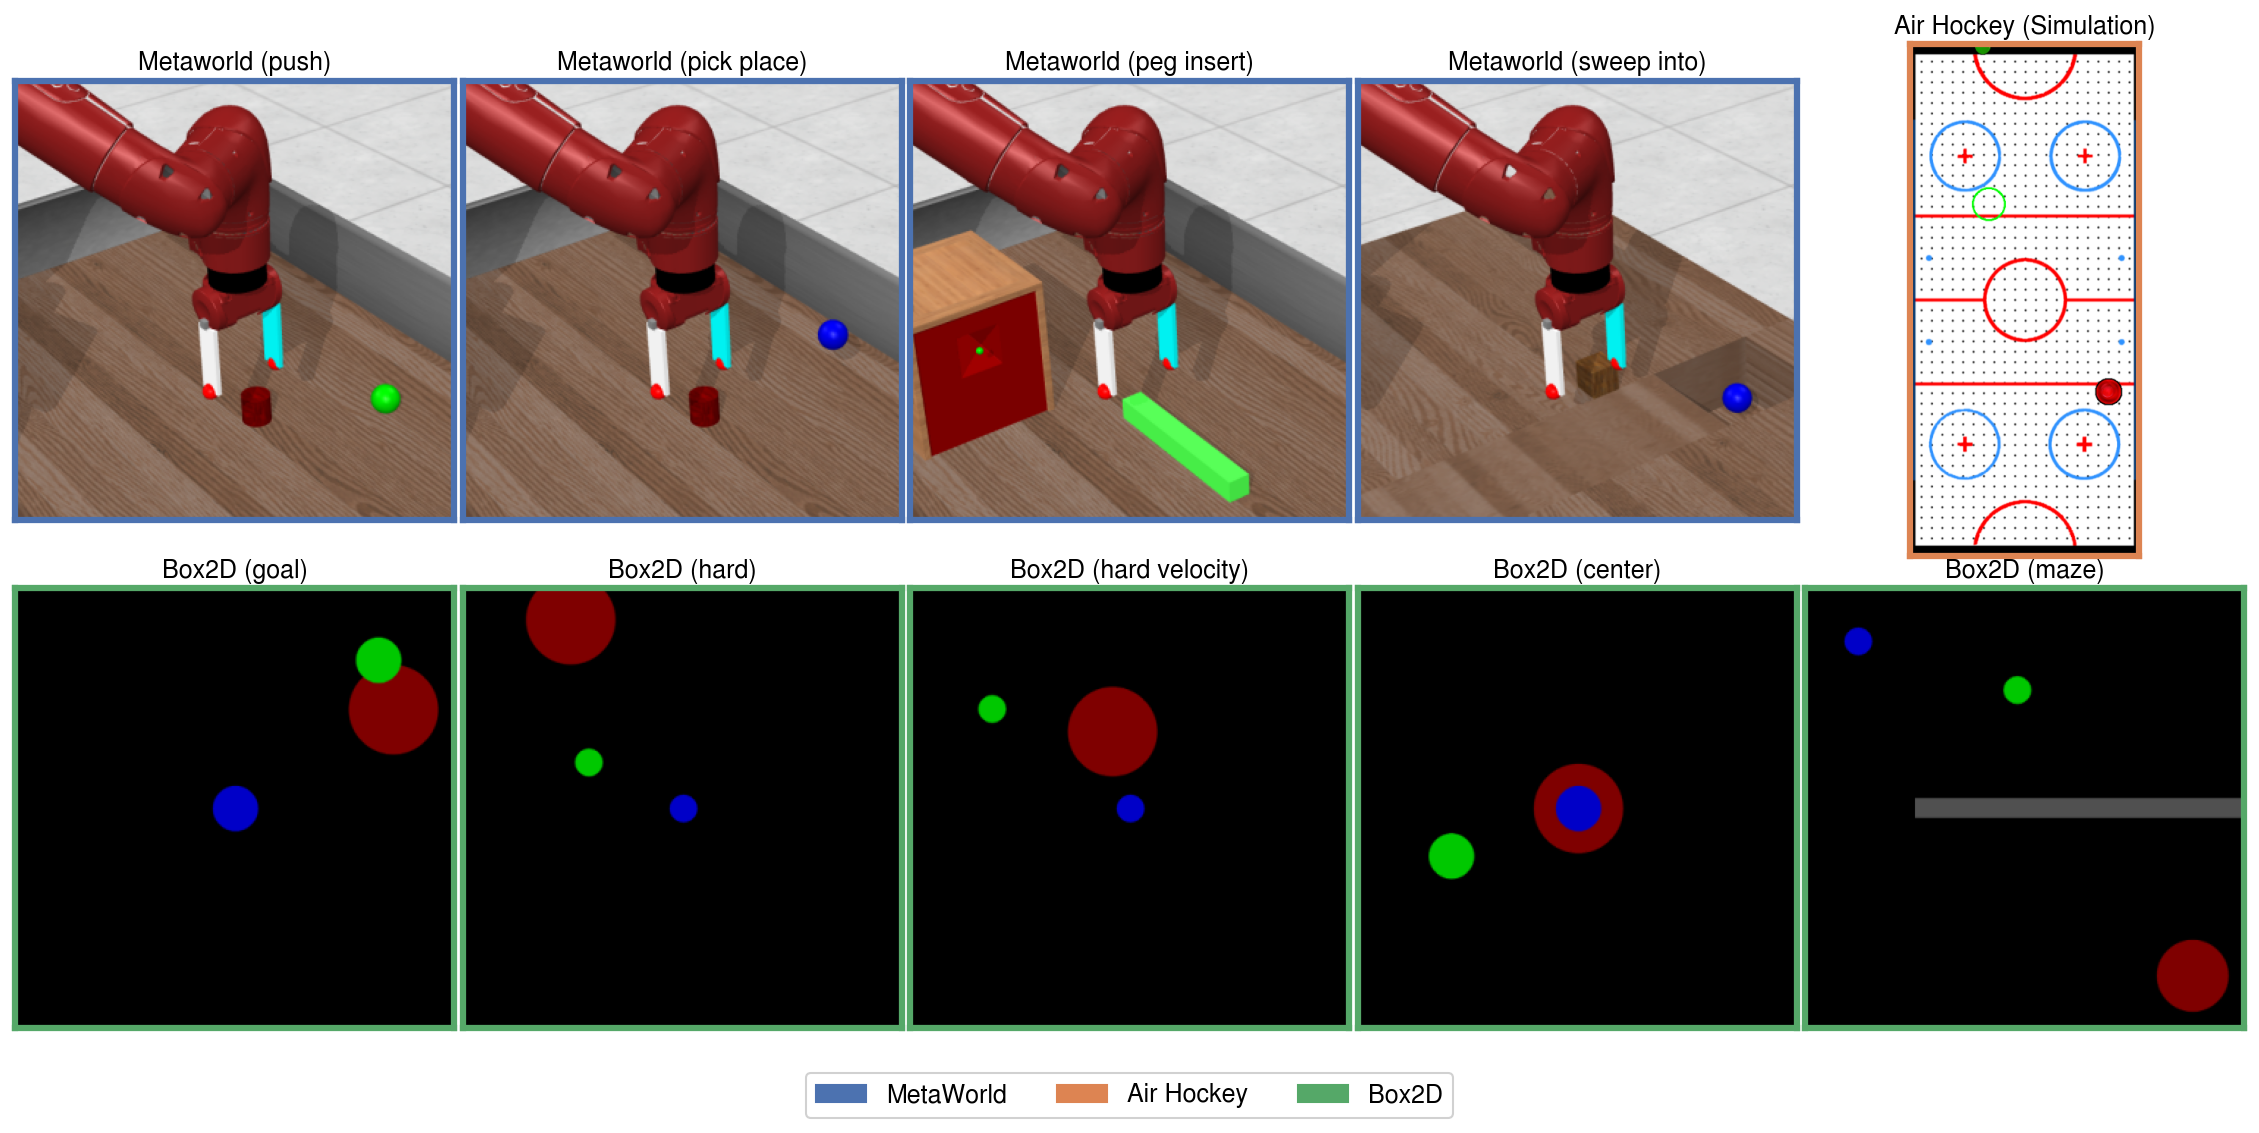
\includegraphics[width=\linewidth]{figure/task_set_figure.png}
%        \caption{Task sets used in the simulation experiments.}
%        \label{fig:task_set}
%    \end{minipage}%
%    \begin{minipage}[t]{0.25\textwidth}
%        \centering
%        \vspace{0pt}
%        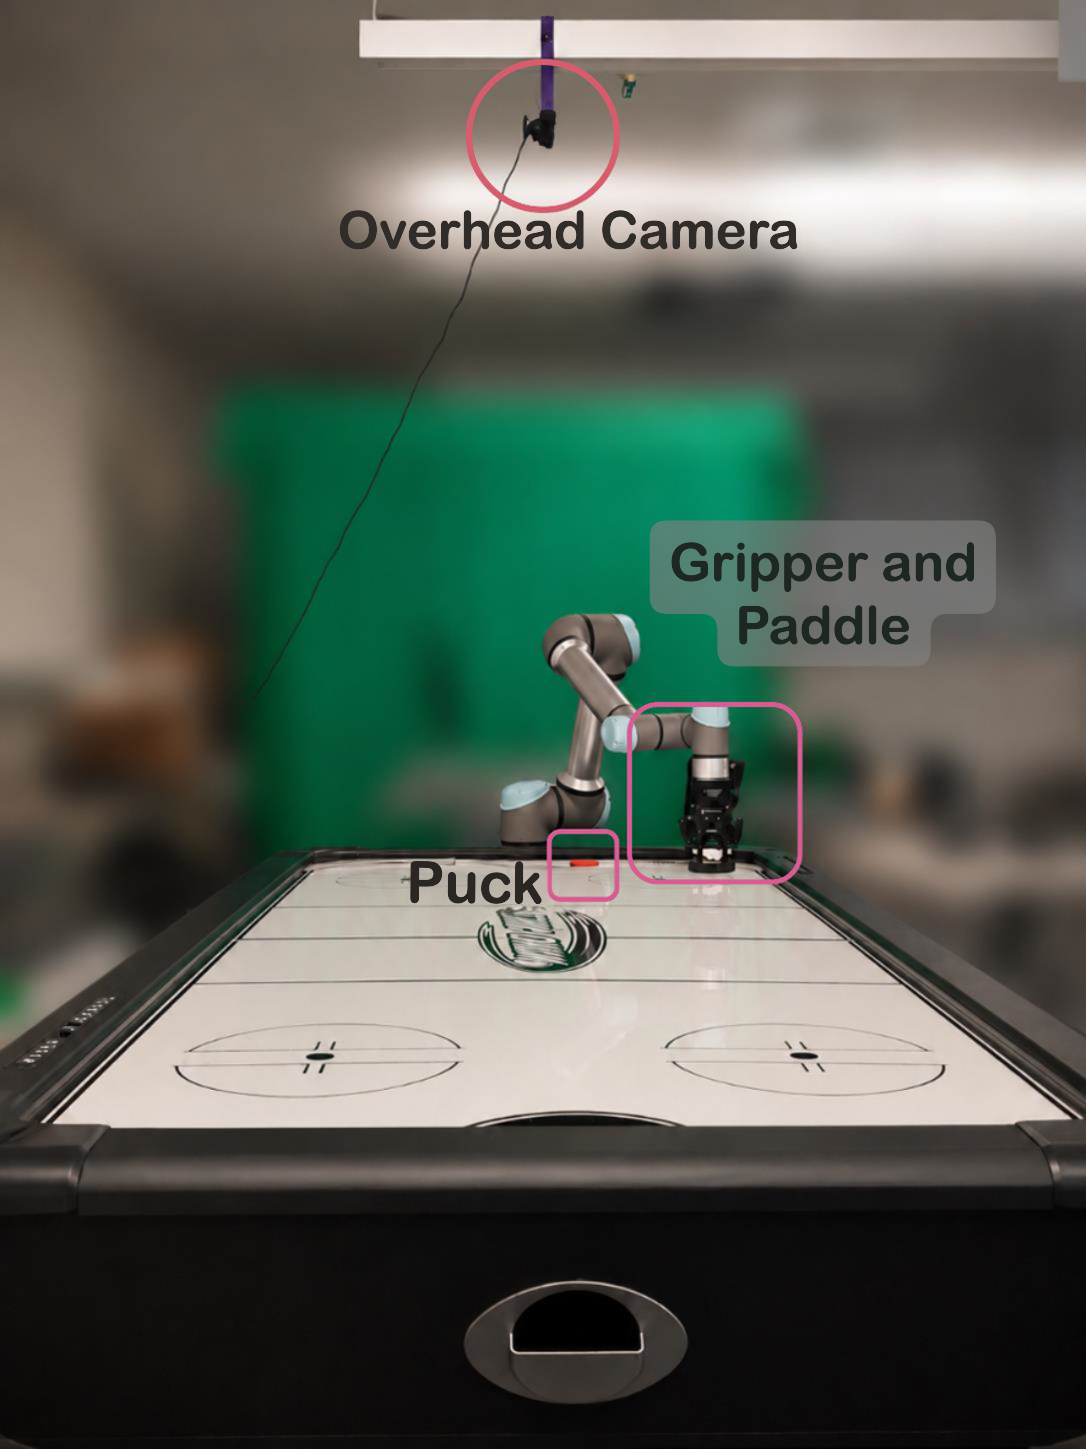
\includegraphics[width=\linewidth]{figure/air_hockey_setup.png}
%        \caption{Real-world robotic air hockey testbed.}
%        \label{fig:real_world_air_hockey_setup}
%    \end{minipage}
%    \vspace{-1em}
%\end{figure}

\paragraph{Experimental Settings}
We evaluate IWR across three groups of interaction-centric environments: 
(i) \textbf{2D Box2D manipulation.} We test IWR with state inputs on five 2D manipulation tasks in Box2D~\citep{catto2026box2d} (Fig.~\ref{fig:task_set}), where the agent controls the blue ball to move the green ball into the red goal region. We report \emph{success ticks}, defined as the number of ticks for which the green ball remains inside the red circle, normalized by 100 ticks, with each episode lasting 200 ticks. 
(ii) \textbf{Robotic manipulation.} We then evaluate IWR on four manipulation tasks: \textsc{Push}, \textsc{Pick-Place}, \textsc{Sweep-Into}, and \textsc{Peg-Insert}, using success rate as the metric. 
(iii) \textbf{Robot air hockey.} Finally, we test IWR in the Air-Hockey simulator~\citep{chuck2024air} using the velocity-observation mode. The task is to hit a falling puck into a small circular goal of radius $r=0.06$, where the paddle starts on the lower board and strikes the puck toward the goal. We further evaluate performance in a consecutive goal-reaching setting. This setting challenges the trained policy to reach as many goals as possible within one minute. Once a goal is reached, a new goal is sampled. We report both the number of successful goal reaches and the survival rate, which indicates whether the puck avoids falling to the bottom within one minute. For sim-to-real transfer, we add observation noise and switch from velocity observations to history-based observations (Sec.~\ref{subsec:real-robot}).
%We first evaluate IWR with state inputs on five 2D manipulation tasks in Box2D \cite{catto2026box2d} (Fig.~\ref{fig:box2d}), where we control the blue ball to move the green ball into the red circle. The metric is success ticks, which indicates how long the green ball stays in the red circle, normalized by 100 ticks, with an episode length of 200 ticks. Then, we evaluate four manipulation tasks: push, pick-place, sweep-into, and peg-insert. The metric is the success rate. Finally, we test the Air-Hockey simulator \cite{chuck2024air} with the velocity-observation mode. We evaluate success rate, and the goal is a small circle with radius $r=0.06$. The puck falls from the top, and the paddle hits the puck on the lower board to hit the goal. For sim-to-real transfer, we add noise and change the observation mode from velocity to history. See Section~\ref{subsec:real-robot} for sim-to-real transfer.

We compare our method against two groups of baselines.
(i) \textbf{Reward-based RL with sparse rewards.}
We evaluate PPO~\citep{schulman2017proximal} and SAC~\citep{haarnoja2018sac}. For SAC, we also consider variants with a hindsight replay buffer~\citep{andrychowicz2017hindsight} and an interaction replay buffer~\citep{chuck2025null}.
(ii) \textbf{Contrastive RL methods.}
We compare against SGCRL~\citep{liu2025singlegoal} and CRTR~\citep{ziarko2026contrastive}. SGCRL and CRTR differ in whether sampling is repeated $R$ times from a single episode. Since our method belongs to the same family as CRTR, we set $R=8$. CRTR can also be viewed as an ablation of our method with interaction-agnostic uniform sampling.
For the CRL family, after the policy first succeeds at goal reaching, we further evaluate consecutive goal reaching: once a goal is reached, the goal position is changed, and the policy continues acting. We report the average consecutive survival rate, defined by whether the puck avoids falling to the bottom, and the goal-reaching count. Each task is repeated over 5 seeds and details are in Appendix~\ref{app:training_setup}.
%We compare our model with the following baselines. First, we compare against reward-based methods using only sparse rewards: 1) PPO \cite{schulman2017proximal}; 2) SAC \cite{haarnoja2018sac}, with a hindsight replay buffer \cite{andrychowicz2017hindsight} and an interaction replay buffer \cite{chuck2025null}. We also compare against the contrastive RL family: 3) SGCRL \cite{liu2025singlegoal} and CRTR \cite{ziarko2026contrastive}. The difference between SGCRL and CRTR is whether sampling is forced to repeat $R$ times from a single episode.
%Note that our method belongs to the same family as CRTR, and we set $R=8$. CRTR can also be considered an ablation with interaction-agnostic uniform sampling. For the CRL family, which first succeeds in goal reaching, we also evaluate consecutive goal reaching with the trained policy, where the goal position changes once it is reached, and we evaluate the average consecutive survival rate (whether the puck falls to the bottom) and the goal-reaching count. For each task, we repeat 5 times. See Appendix~\ref{app:training_setup} for training details.
%\begin{wrapfigure}{r}{0.33\textwidth}
%\vspace{-1em}
 %   \centering
 %   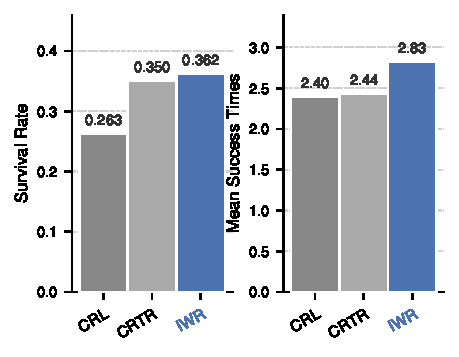
\includegraphics[width=\linewidth]{figure/bar_chart.pdf}
  %  \vspace{-0.8em}
  %  \caption{\small Your figure caption.}
  %  \vspace{-1em}
  %  \label{fig:bar}
%\end{wrapfigure}

% \usepackage{subcaption}

%\begin{figure}[t]
%    \centering
%    \includegraphics[width=0.55\linewidth]{figures/air_hockey_real_transfer_curve.pdf}
%    \caption{
%    Sim-to-real transfer performance on robot air hockey.
%    IWR achieves higher success rate than CRL, CRTR, and sparse-reward RL baselines under the real-transfer setting.
%    Shaded regions indicate variation across runs.
%    }
%    \label{fig:air_hockey_real_transfer_curve}
%\end{figure}

\begin{figure*}[t]
    \centering
    \begin{subfigure}{0.33\textwidth}
        \centering
        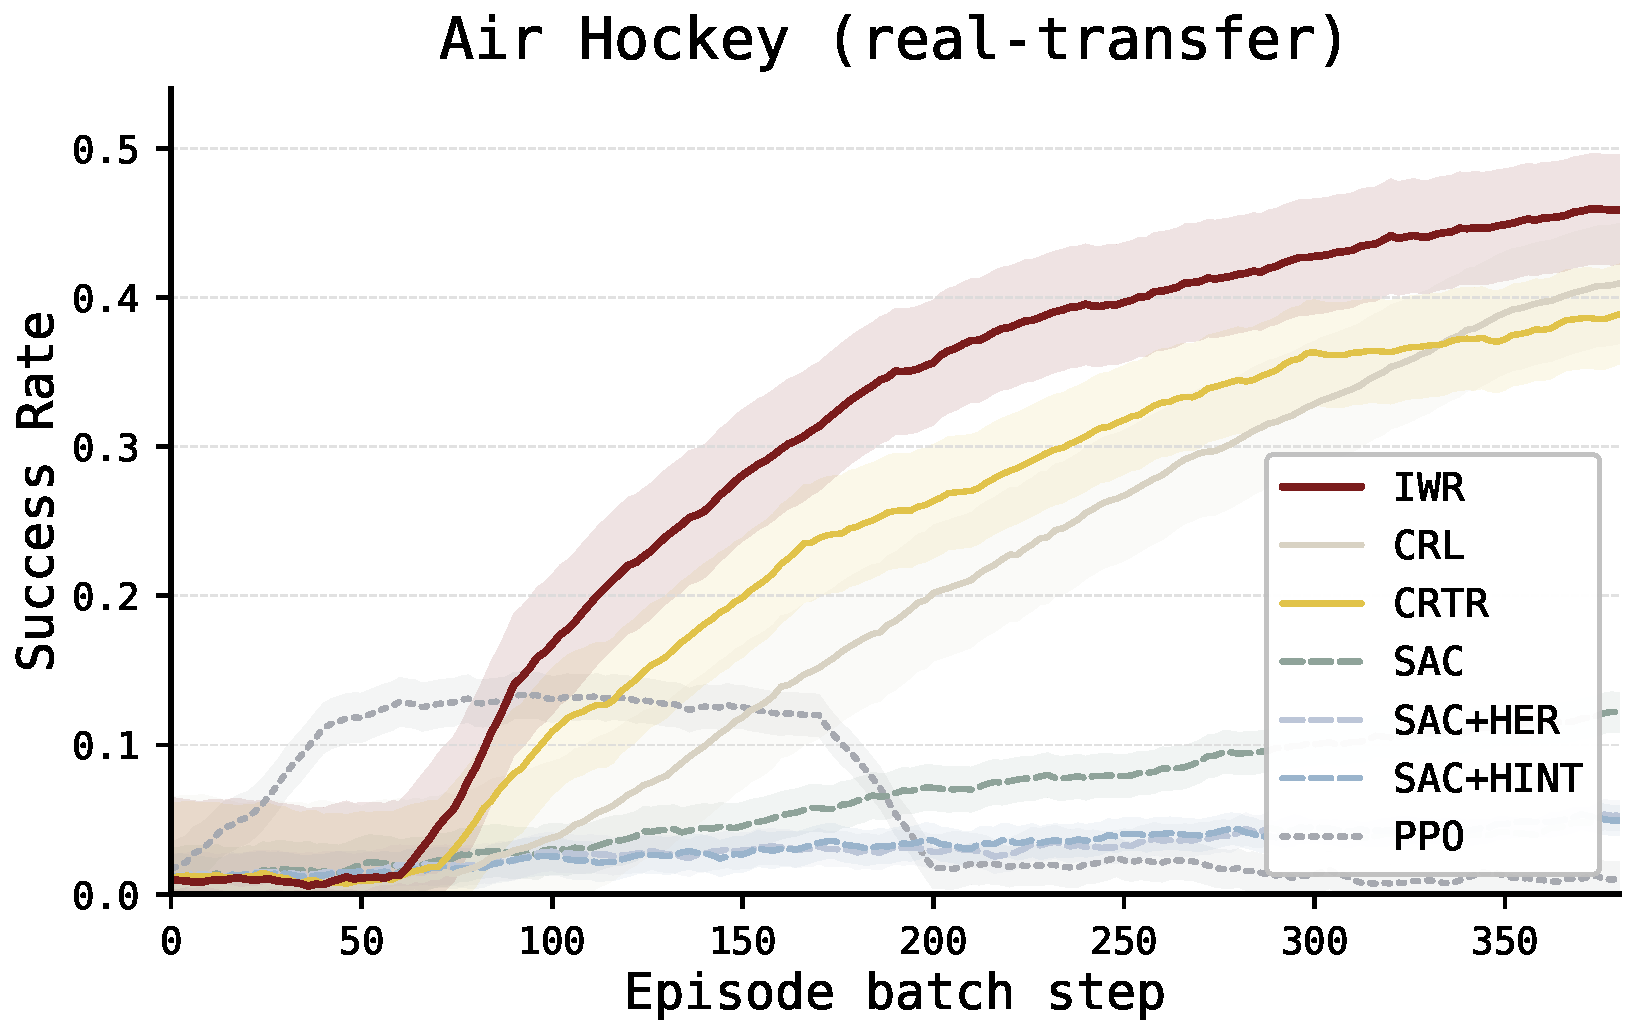
\includegraphics[width=\linewidth]{figure/air_hockey_survival_rate.pdf}
        \caption{Training curve.}
        \label{fig:air_hockey_real_transfer_curve}
    \end{subfigure}
    \hfill
    \begin{subfigure}{0.41\textwidth}
        \centering
        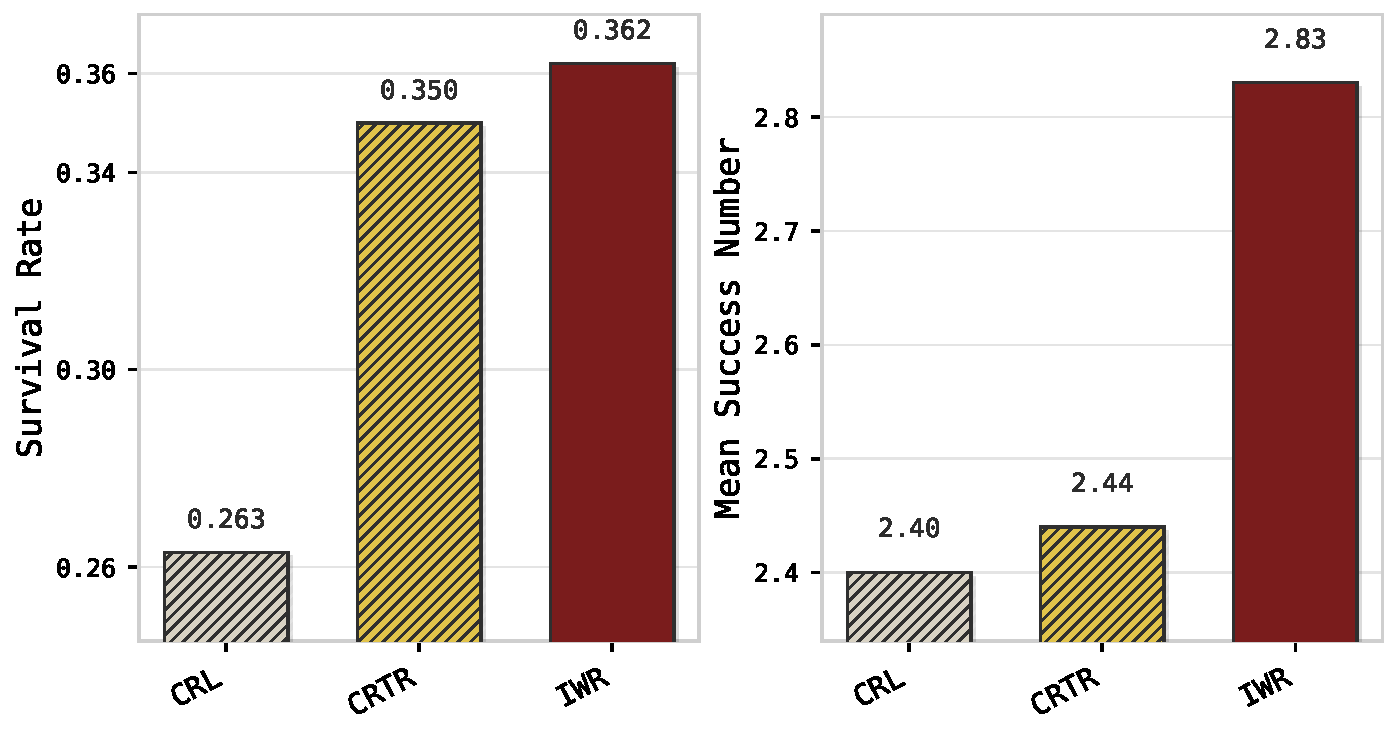
\includegraphics[width=\linewidth]{figure/air_hockey_success_times.pdf}
        \caption{Consecutive evaluation.}
        \label{fig:air_hockey_consecutive_eval}
    \end{subfigure}
    \hfill
    \begin{subfigure}{0.2\textwidth}
        \centering
        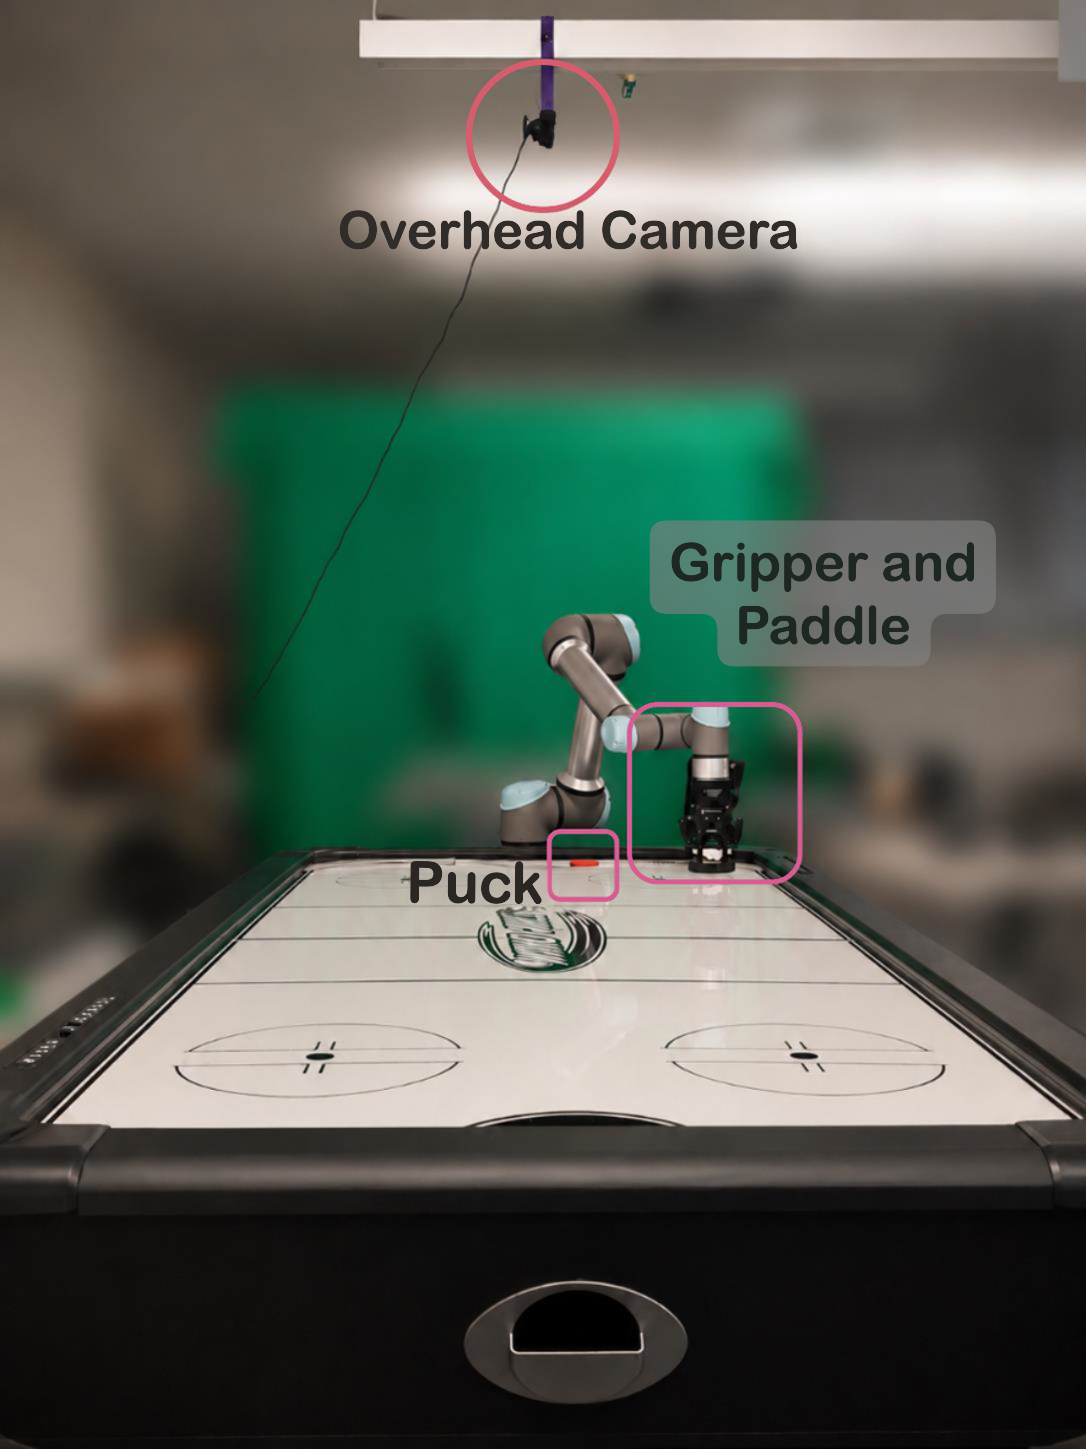
\includegraphics[width=\linewidth]{figure/air_hockey_setup.png}
        \caption{Real robot setup.}
    \label{fig:air_hockey_setup}
    \end{subfigure}
    \caption{
    \textbf{Air hockey real-transfer}.    (a) Training performance in simulation under the real-transfer setting.
    (b) Consecutive evaluation after training in simulator.
    (c) Real robot air hockey setup.
    }
\label{fig:air_hockey_real_transfer}
    \vspace{-0.6cm}
\end{figure*}

\textbf{Results} 
Table~\ref{tab:main1} reports the best average performance of all algorithms. 
The reward-free \textbf{CRL family outperforms the PPO algorithm and SAC family}, even when SAC is augmented with hindsight replay and interaction replay. The reward-based method has no success on MetaWorld and Air Hockey Real Robot. This agrees with previously observed~\citep{eysenbach2021clearning} comparative results.
% efficacy of self-improvement through contrastive representations, which provides better estimation in sparse-reward settings than Bellman-backup-based Q-value estimation.
IWR outperforms prior methods on most tasks, with an average gain of 19.8\%. 
A key pattern is that the gains are \textbf{largest when interaction and goal-reaching signals are sparse}, supporting our hypothesis that IWR amplifies interaction-relevant supervision and learns a better goal-reaching energy landscape.

In \texttt{\textbf{Box2D}}, precise-control tasks require the agent to keep the green ball near the goal center, demanding both exploration and accurate interaction modeling. The hard variants make the objects smaller, further reducing successful interaction signals; here IWR yields larger gains. In the hard-velocity setting, random initial velocities occasionally create early successes, so the relative improvement is smaller but still substantial. This shows that IWR is especially useful when interaction events are rare but necessary for success.
\texttt{\textbf{Metaworld}} shows a similar trend. In \textsc{Push} and \textsc{Sweep-Into}, random behavior can sometimes succeed, and the goal can be reached through multiple strategies, such as pushing or stabbing the object into the goal. In contrast, \textsc{Pick-Place} requires precise long-horizon interaction, since the policy must grasp and carry the object. IWR achieves a much larger gain in this task, suggesting that interaction-weighted sampling extends beyond the simplified one-step setting in Proposition~\ref{prop:endpoint-energy-error} to hybrid dynamics with repeated interaction propagation, e.g., terms of the form $A_1^k$.
For \texttt{\textbf{air hockey}}, the single-goal success-rate gain is modest, but Fig.~\ref{fig:air_hockey_real_transfer_curve} shows great improvements in real-transfer setting, which includes noise and discontinuous observations. This indicates IWR would be consistent when the environment is noisy, and the learned policy and critic is more generalizable with higher sample coverage near interaction.

Fig.~\ref{fig:air_hockey_consecutive_eval} shows the evaluation on consecutive goal-hitting evaluation. This indicates that IWR improves not only isolated successes, but also the robustness and precision of interaction control. The effect is even more pronounced in the real-world setting, as discussed in Sec.~\ref{subsec:real-robot}.

\definecolor{ourscol}{RGB}{255,238,238}
\definecolor{gainrow}{RGB}{255,248,246}
\definecolor{strongcell}{RGB}{255,220,220}

\begin{table*}[t]
\centering
\small
\setlength{\tabcolsep}{4pt}
\caption{
Success rates over Air Hockey, Box2D, and MetaWorld tasks.
Light red rows highlight interaction-centric tasks where IWR provides larger gains.
}
\label{tab:main1}
\resizebox{\textwidth}{!}{%
\begin{tabular}{lrrrrrrr}
\toprule
Task & PPO & SAC & SAC+HER & SAC+HINT & CRL & CRTR & IWR (Ours) \\
\midrule
Air Hockey (Simulation) & 0.617 & 0.145 & 0.398 & 0.422 & 0.695 & 0.727 & \cellcolor{ourscol}\textbf{0.742 (+2.1\%)} \\
Air Hockey (real-transfer) & 0.160 & 0.215 & 0.129 & 0.125 & 0.477 & 0.465 & \cellcolor{ourscol}\textbf{0.500 (+4.8\%)} \\
\rowcolor{gainrow}
Air Hockey (Real Robot) & 0/20 & 0/20 & 0/20 & 0/20 & 5/20 & 2/20 & \cellcolor{strongcell}\textbf{12/20 (+140.0\%)} \\

\midrule
Box2D (center) & 0.086 & 0.058 & 0.088 & 0.088 & 0.278 & 0.274 & \cellcolor{ourscol}\textbf{0.288 (+3.6\%)} \\
Box2D (goal) & 0.089 & 0.046 & 0.086 & 0.064 & 0.450 & 0.558 & \cellcolor{ourscol}\textbf{0.709 (+27.1\%)} \\
\rowcolor{gainrow}
Box2D (hard) & 0.060 & 0.042 & 0.064 & 0.076 & 0.317 & 0.365 & \cellcolor{strongcell}\textbf{0.565 (+54.8\%)} \\
Box2D (hard velocity) & 0.148 & 0.149 & 0.152 & 0.139 & 0.387 & 0.377 & \cellcolor{ourscol}\textbf{0.436 (+12.7\%)} \\
Box2D (maze) & 0.033 & 0.012 & 0.031 & 0.035 & 0.217 & 0.206 & \cellcolor{ourscol}\textbf{0.223 (+2.8\%)} \\

\midrule
MetaWorld (peg insert) & 0.000 & 0.000 & 0.000 & 0.000 & 0.430 & 0.367 & \cellcolor{ourscol}\textbf{0.438 (+1.9\%)} \\
\rowcolor{gainrow}
MetaWorld (pick place) & 0.000 & 0.000 & 0.004 & 0.000 & 0.266 & 0.305 & \cellcolor{strongcell}\textbf{0.570 (+86.9\%)} \\
MetaWorld (push) & 0.000 & 0.000 & 0.004 & 0.000 & 0.699 & \textbf{0.750} & \cellcolor{ourscol}0.730 \\
MetaWorld (sweep into) & 0.000 & 0.004 & 0.020 & 0.004 & 0.805 & 0.910 & \cellcolor{ourscol}\textbf{0.926 (+1.8\%)} \\

\midrule
Average IWR improvement &  &  &  &  &  &  & \cellcolor{strongcell}\textbf{+19.8\%} \\
\bottomrule
\end{tabular}%
}
\end{table*}
% % \begin{table}[t]
% \centering
% \small
% \setlength{\tabcolsep}{8pt}
% \caption{Air Hockey one-minute consecutive-goal evaluation on the r0.06 velocity setting. Each entry reports the best checkpoint for that metric over the local checkpoint sweep, averaged over five training seeds and evaluated with 16 rollout seeds per checkpoint.}
% \label{tab:air_hockey_consecutive_survival}
% \resizebox{\linewidth}{!}{%
% \begin{tabular}{lrrrr}
% \toprule
% Method & Survival Rate & Mean success times\\
% \midrule
% CRL & 0.2625 & 2.4000 \\
% CRTR & 0.3500 & 2.4375 \\
% \textbf{IWR (Ours)} & \textbf{0.3625} & \textbf{2.8250} \\
% \midrule
% \textbf{IWR improvement over second best} & \textbf{+3.6\%} & \textbf{+15.9\%}\\
% \bottomrule
% \end{tabular}%
% }
% \end{table}
%\vspace{-0.8em}
\subsection{Real-Robot Experiment}
%\vspace{-0.8em}
\label{subsec:real-robot}
\paragraph{Experimental Settings} In this work, we utilize the setting of \citet{chuck2024robot} as seen in Fig.~\ref{fig:real_world_air_hockey_setup} with a sim-to-real pipeline with domain randomization to transfer policies from the 2D simulator to a UR5e robot on one end of an air hockey table (see Fig.~\ref{fig:paired_sim_real}). The state space is unified between both 2D and 3D through puck detection and coordinate frame transformation. No training is performed on the real robot setup---all policies are transferred sim-to-real, and evaluated on a grid of $4\times5$ goals. Additional robot details, especially the sim-to-real pipeline, can be found in Appendix~\ref{app:real_setup}.
\vspace{-0.8em}
\paragraph{Results} As we see in Table~\ref{tab:main1}, the success rate for \methodshort{} significantly exceeds that of the other methods ($140\%$ more success), even though the gap in simulation (Air Hockey real-transfer) is significantly smaller ($5\%$ increase). We believe this is because when transferring sim-to-real, the qualitative aspects of the policy, that is, how it induces interactions, make a larger difference. Because \methodshort{} emphasizes greater representation capacity for interactions, it makes contact with the puck more consistently, and with greater upward force. This results in more overall strikes, which significantly boosts the performance. Other comparable methods make contact with the puck only once, resulting in unrecoverable failures. Nonetheless, the performance improvement of \methodshort{} is substantial, suggesting that by focusing on interactions, it learns a more robust policy. This is qualitatively visible in the visualizations of the policy performance found in Appendix Figures~\ref{fig:crtr-paired}-\ref{fig:sgcrl-render-paired}.


\begin{figure}
    \centering
    \vspace{-1em}
    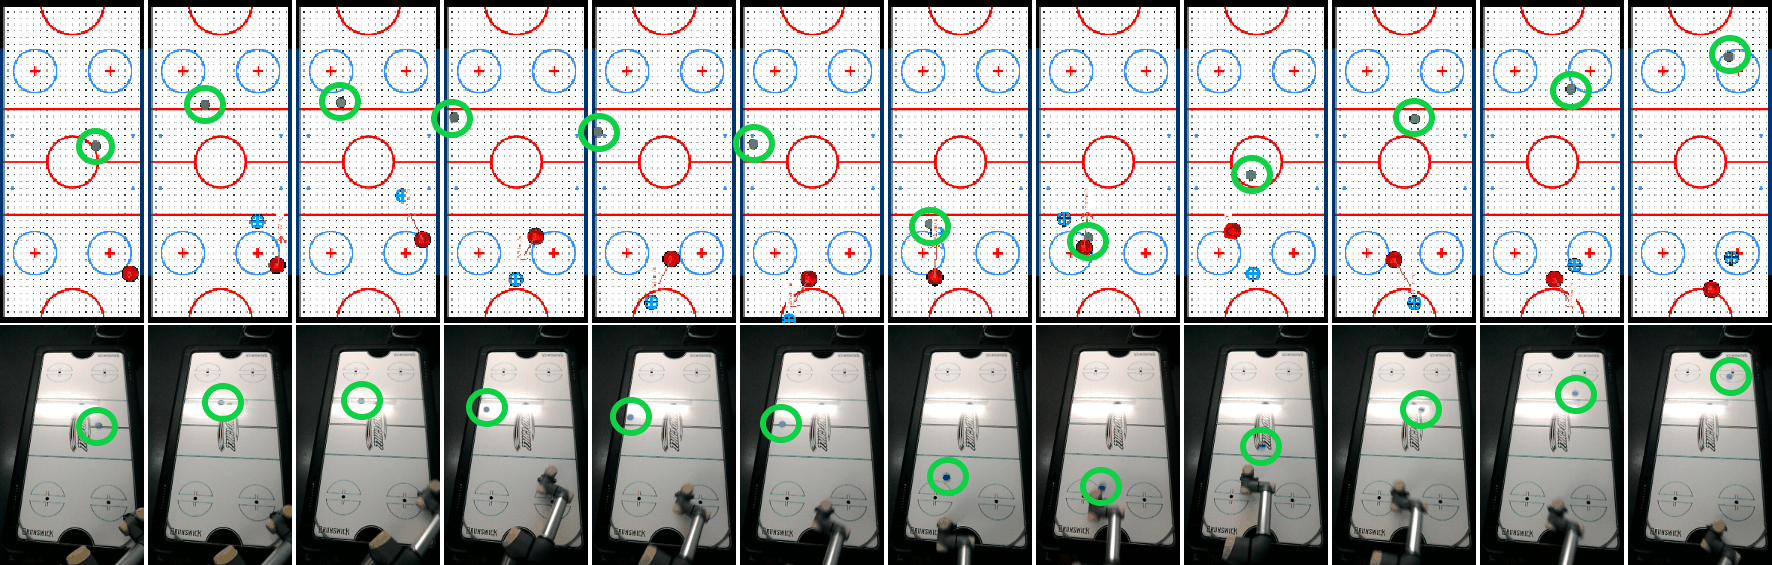
\includegraphics[width=0.98\textwidth]{figure/paired_sim_real.png}
    \caption{
    2D sim paired with corresponding real frames. Puck emphasized with green circle.
    }
    \label{fig:paired_sim_real}
    \vspace{-1em}
\end{figure}



